\section{Technologies}\label{sec:technologies}

The languages and technologies used are mainly those imposed by the already existing Åboat infrastructure, however given the decoupling factor of the components in the software stack, we are free to choose the technology we use for the VRGP service and the MOC.
\\\\
For the vessel-side adapter (i.e. the VRGP adapter running inside an OpenDLV microservice), the technologies used are:

\begin{itemize}
	\item C++ and OpenDLV (microservices solution), built on top of the Cluon library
	\item WebSockets and WebRTC (communication protocols for streams of data and video over the internet)
	\item Docker (container solution)
	\item Raspberry Pi, LIDAR, GPS, radar, compass, and other existing hardware equipment
\end{itemize}

\noindent
For the VRGP service that runs on the vessel-side, the technologies used are:

\begin{itemize}
	\item Java and Spring Boot
	\item WebSockets and WebRTC (communication protocols for streams of data and video over the internet)
	\item Docker (container solution)
\end{itemize}

\noindent
For the MOC that runs on the shore-side, the technologies used are:

\begin{itemize}
	\item Java and Spring Boot
	\item WebSockets and WebRTC (communication protocols for streams of data and video over the internet)
	\item Docker (container solution)
\end{itemize}

\noindent
Additionally, there is going to be a web interface as a way to test the VRGP connection to the vessel. Åboat currently has a web interface capable of streaming some data from the vessel to the shore, however we built our own interface as a way to properly integrate all the information from the VRGP specification. The technologies that will be used in this regard are:

\begin{itemize}
	\item Web technologies (HTML, CSS, JavaScript)
	\item WebSockets and WebRTC (communication protocols for streams of data and video over the internet)
\end{itemize}

\section{Components}\label{sec:components}

In the following sections, every component will be explained in more detail. The general interconnection between components is shown in figure \ref{fig:vrgp-architecture}.

\subsection{VRGP service}

The VRGP service is the main component of the software stack. It is the implementation of the VRGP specification. The service is meant to be independent and universal. This means that with a small interface (called an adapter), every vessel should be able to run it, anywhere.
\\\\
The VRGP service is responsible for the communication between the vessel (which is represented in the software stack as the adapter), and the MOC, running on the shore-side.

\subsection{MOC backend}

The MOC backend is responsible for communicating with an arbitrary amount of vessels following the VRGP specification. It represents the shore-side center of operation. The MOC backend itself exposes an interface (an API), which can be used by a frontend to display the information.
\\\\
A class-diagram depicting the MOC backend structure is shown in figure \ref{fig:moc-class-diagram}.

\begin{figure}[ht]
	\centering
	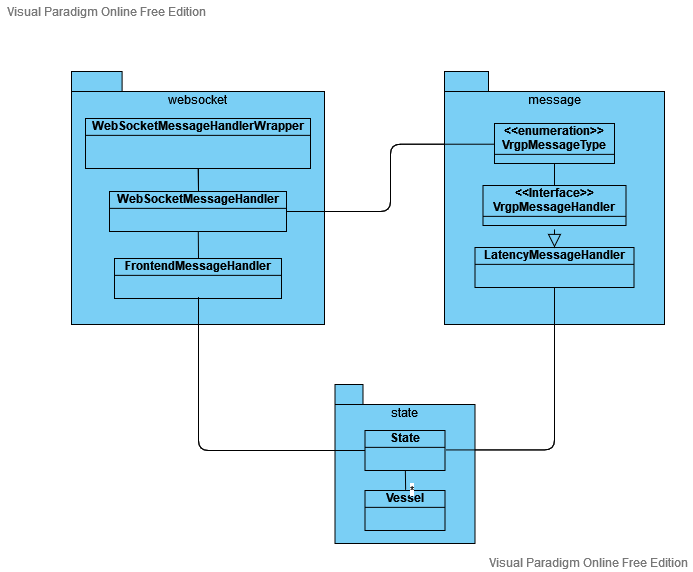
\includegraphics[width=\linewidth]{diagrams/ClassDiagramMOC}
	\caption{MOC class diagram}
	\label{fig:moc-class-diagram}
\end{figure}

\subsection{MOC frontend}

The MOC frontend is responsible for displaying the information from the MOC backend to human operators. All the functionality of the VRGP specification can be accessed from the MOC frontend. This means information about any specific vessel connected to the MOC can be visualized, and arbitrary commands or guidance messages can be sent from the frontend.

\subsection{VRGP - Åboat adapter}

The VRGP adapter's role is to translate calls between the Åboat and the VRGP service. This is needed because the Åboat already has an existing architecture. Thus it is not possible to integrate the VRGP service directly into its architecture in an easy way. More generally, the service shouldn't be separately built for every different vessel, but rather should be built independently of each vessel, and then \textbf{adapted} accordingly. The role of the adapter is then that of a "translator", to integrate itself into existing architectures and establish a channel between vessels and the VRGP service. Such an adapter is easy to build, and only requires minimal work to be done.
\\\\
Of course, a vessel can be built around the VRGP service itself, in which case there would be no need for an adapter at all. The adapter itself is a way to provide backwards-compatibility, or to give a vessel the possibility to have more than one protocol through which to communicate.
\\\\
The adapter class diagram can be seen in figure \ref{fig:adapter-class-diagram}.

\begin{figure}[ht]
	\centering
	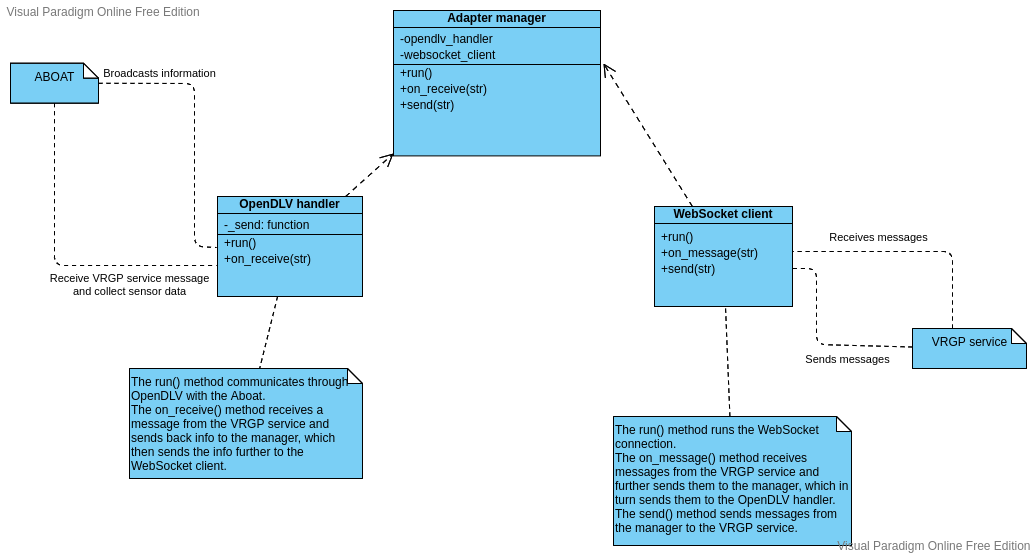
\includegraphics[width=\linewidth]{diagrams/ClassDiagramAdapter}
	\caption{Adapter class diagram}
	\label{fig:adapter-class-diagram}
\end{figure}
